%% LyX 2.0.7 created this file.  For more info, see http://www.lyx.org/.
%% Do not edit unless you really know what you are doing.
\documentclass[11pt,twocolumn]{article}
\usepackage[utf8]{inputenc}
\usepackage{graphicx}

\makeatletter
%%%%%%%%%%%%%%%%%%%%%%%%%%%%%% User specified LaTeX commands.








\title{Structured Merge Tool for the PDStore Database }
\author{Kartik Andalam, Raoul D'Cunha, Shreya Shah }
\date{March 2014}

















\makeatother

\begin{document}
\maketitle

%\twocolumn



\section{Abstract}

Software merging is a necessity for large-scale software development
and while there are many code version systems to help with this, many
of them don't take the structure of the code into account. We propose
to develop a merge tool that will utilise the PDStore%
\footnote{PDStore is a Triplestore database developed at the University of Auckland%
} database to maintain and analyse the structure of the data.

The aim of the tool is to utilise information related to the structure
of a file stored in PDStore and highlight the conflicts that arise
in merging. The proposal highlights the requirements, milestones and
possible evaluation methods for the research project.


\section{Motivation}

%Today's code version systems are based on textual comparisons. Being
%textual based means that they do not understand the structure of the
%code, and as a result the tools are unable to fully assist the developer
%with code merging. This gave a reason to utilise the extra information
%that can aid in the merging.


Developing a merge tool that maintains information in a structured
form gives scope to improve the way conflicts and changes are shown.
This motivated us to explore the effectiveness and usability of such
merge tools and how they compare to existing merge tools.


\section{Related Work}

\cite{SemanticDiff} describes a tool called “Semantic diff” and techniques
used in that tool to show the effect of modifications. The tool aims
at providing the user with a summarised report of semantic changes
between two versions of a procedure, and focuses on minimising any
spurious differences such as renaming local variables. While the tool
provides knowledge of variable dependences within a procedure, it
is not very helpful when considering an entire program because the
tool does not maintain any relationship between method invocation
and method definition.

In \cite{XMLMerge} a technique for performing a 3 way structured
XML merge is described. The technique involves defining merge rules
derived from common use cases of XML editing. While there are similar
problems, a few differences exist. By the nature of XML, the local
structure is important. The rules made in \cite{XMLMerge} become
invalid for flexible structured data such as code. We will utilise
PDStore and abstract the tool in such a way that it can be used to
assist in merging a variety of structured documents.

The system described in \cite{finegraned} utilises fine-grained revision
control functionality to keep track of program modifications and support
merging. The merge tool of this system defines rules using the user’s
past revisions to suggest a merged result to the user and also allows
the user to make changes to the temporary result. While the tool automatically
generates a merged result, the basis of these rules are related to
user configuration rather than the merge tool defining the rules.

\cite{mergegraph} describes the problems associated with common textual
based merging. It proposes a solution that can be applied to software
artefacts of different types. The solution involves representing information
with extra information such as namespaces appended with UIDs. Once
the data is represented in this special structure, the job of analysing
two structures should be made easier.


\section{Requirements}

A successful execution of the research endeavour should meet the following
requirements: 
\begin{enumerate}
\item Visually show the changes between two transactions with the use of
tree views 
\item Allow the user to specify what should exist in the new state after
merge. Merge in this case is combining two states of a store to produce
a third state 
\item Offers the ability to perfrom a three way merge 
\item Integrate into PDStore application 
\item Evaluate the usability of the tool comparing with existing merge tools 
\end{enumerate}

\section{Design and Implementation}

The underlying technology used in the proposed method involves using
PDStore to form a structured view of the code. The merging logic will
be written in Scala, while the GUI will be designed in Swing.

Figure 1 is an example that illustrates a possible GUI for three way
merging involving PD Tree Views. The title string belonging to the
LOTR book in the My book library database has differing values in
each of the three existing versions(Base, Version A and Version B).
We hope to colour code information such as modified items and/or items
in conflict to help better inform the user of the types of changes.
The user can select items from different versions to be included in
the merged representation by clicking on the checkbox beside the items.

\begin{figure}
\centering{}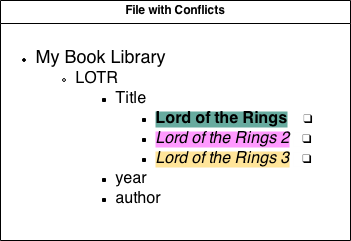
\includegraphics[scale=0.44]{Diagramv2}\caption{Proposed GUI for merge tool}
\end{figure}



\section{Evaluation}

This evaluation will consist of usability testing and comparative
analysis with existing merge tools.

As part of the usability testing, paper prototypes will be used to
evaluate the feasibility of the design of the User Interface of our
tool. This study will reveal both fundamental and minor flaws in the
UI that would need to be fixed before the final milestone. Specific
scenarios will be constructed outlining various use cases that will
then be run through by the participants on multiple different UI designs.
The participants will be asked to think out loud, so that their thought
process can be observed and evaluated. Feedback will then be collected
from the participants at the end through the use of a questionnaire
which will then be used to measure the usefulness of each design.

Any identified flaws will then be corrected and the test will then
be undertaken again so as to verify that the flaws are indeed fixed.

The comparative analysis will consist of test cases outlining major
scenarios that will be laid out at the start of the project and will
later be run against existing merge tools and our developed merge
tool. The outcome of these test scenarios will help determine the
effectiveness of the tools under different scenarios


\section{Project Plan}

Listed below are the three milestones for this project %\newline adding a new line puts too much space over here

\begin{description}
\item [{Milestone One:}] Visually show the effect of a transaction


Visually show the changes before and after a transaction. Changes
should be displayed in terms of roles and relations. \\
 \textbf{Due Date:} 15th April 2014

\item [{Milestone Two:}] Able to perform Three-way merge


This involves creating a UI such that the user can select the links/relations
that will exist the merged version. \\
 \textbf{Due Date:} 30th April 2014

\item [{Milestone Three:}] Integrate the functionality into PDHistoryViewer
application


Integrating the added functionality will allow us to conduct our evaluation
on users. This will be key in determining the usefulness and effectiveness
of the changes.\\
 \textbf{Due Date:} 12th May 2014

\end{description}
 \bibliographystyle{plain}
\bibliography{myBib}

\end{document}
